\documentclass{article}

\usepackage{graphicx}
\usepackage{tikz}
\usepackage{tikzsymbols}
\usetikzlibrary{calc,patterns,shapes.geometric}
\pagestyle{empty}
\usepackage[margin=0pt]{geometry}
\geometry{papersize={14in,12in}}

\def\centerarc[#1](#2)(#3:#4:#5){\draw[#1] ($(#2)+({#5*cos(#3)},{#5*sin(#3)})$) arc (#3:#4:#5);}

\begin{document}
	\begin{figure}
		\centering
		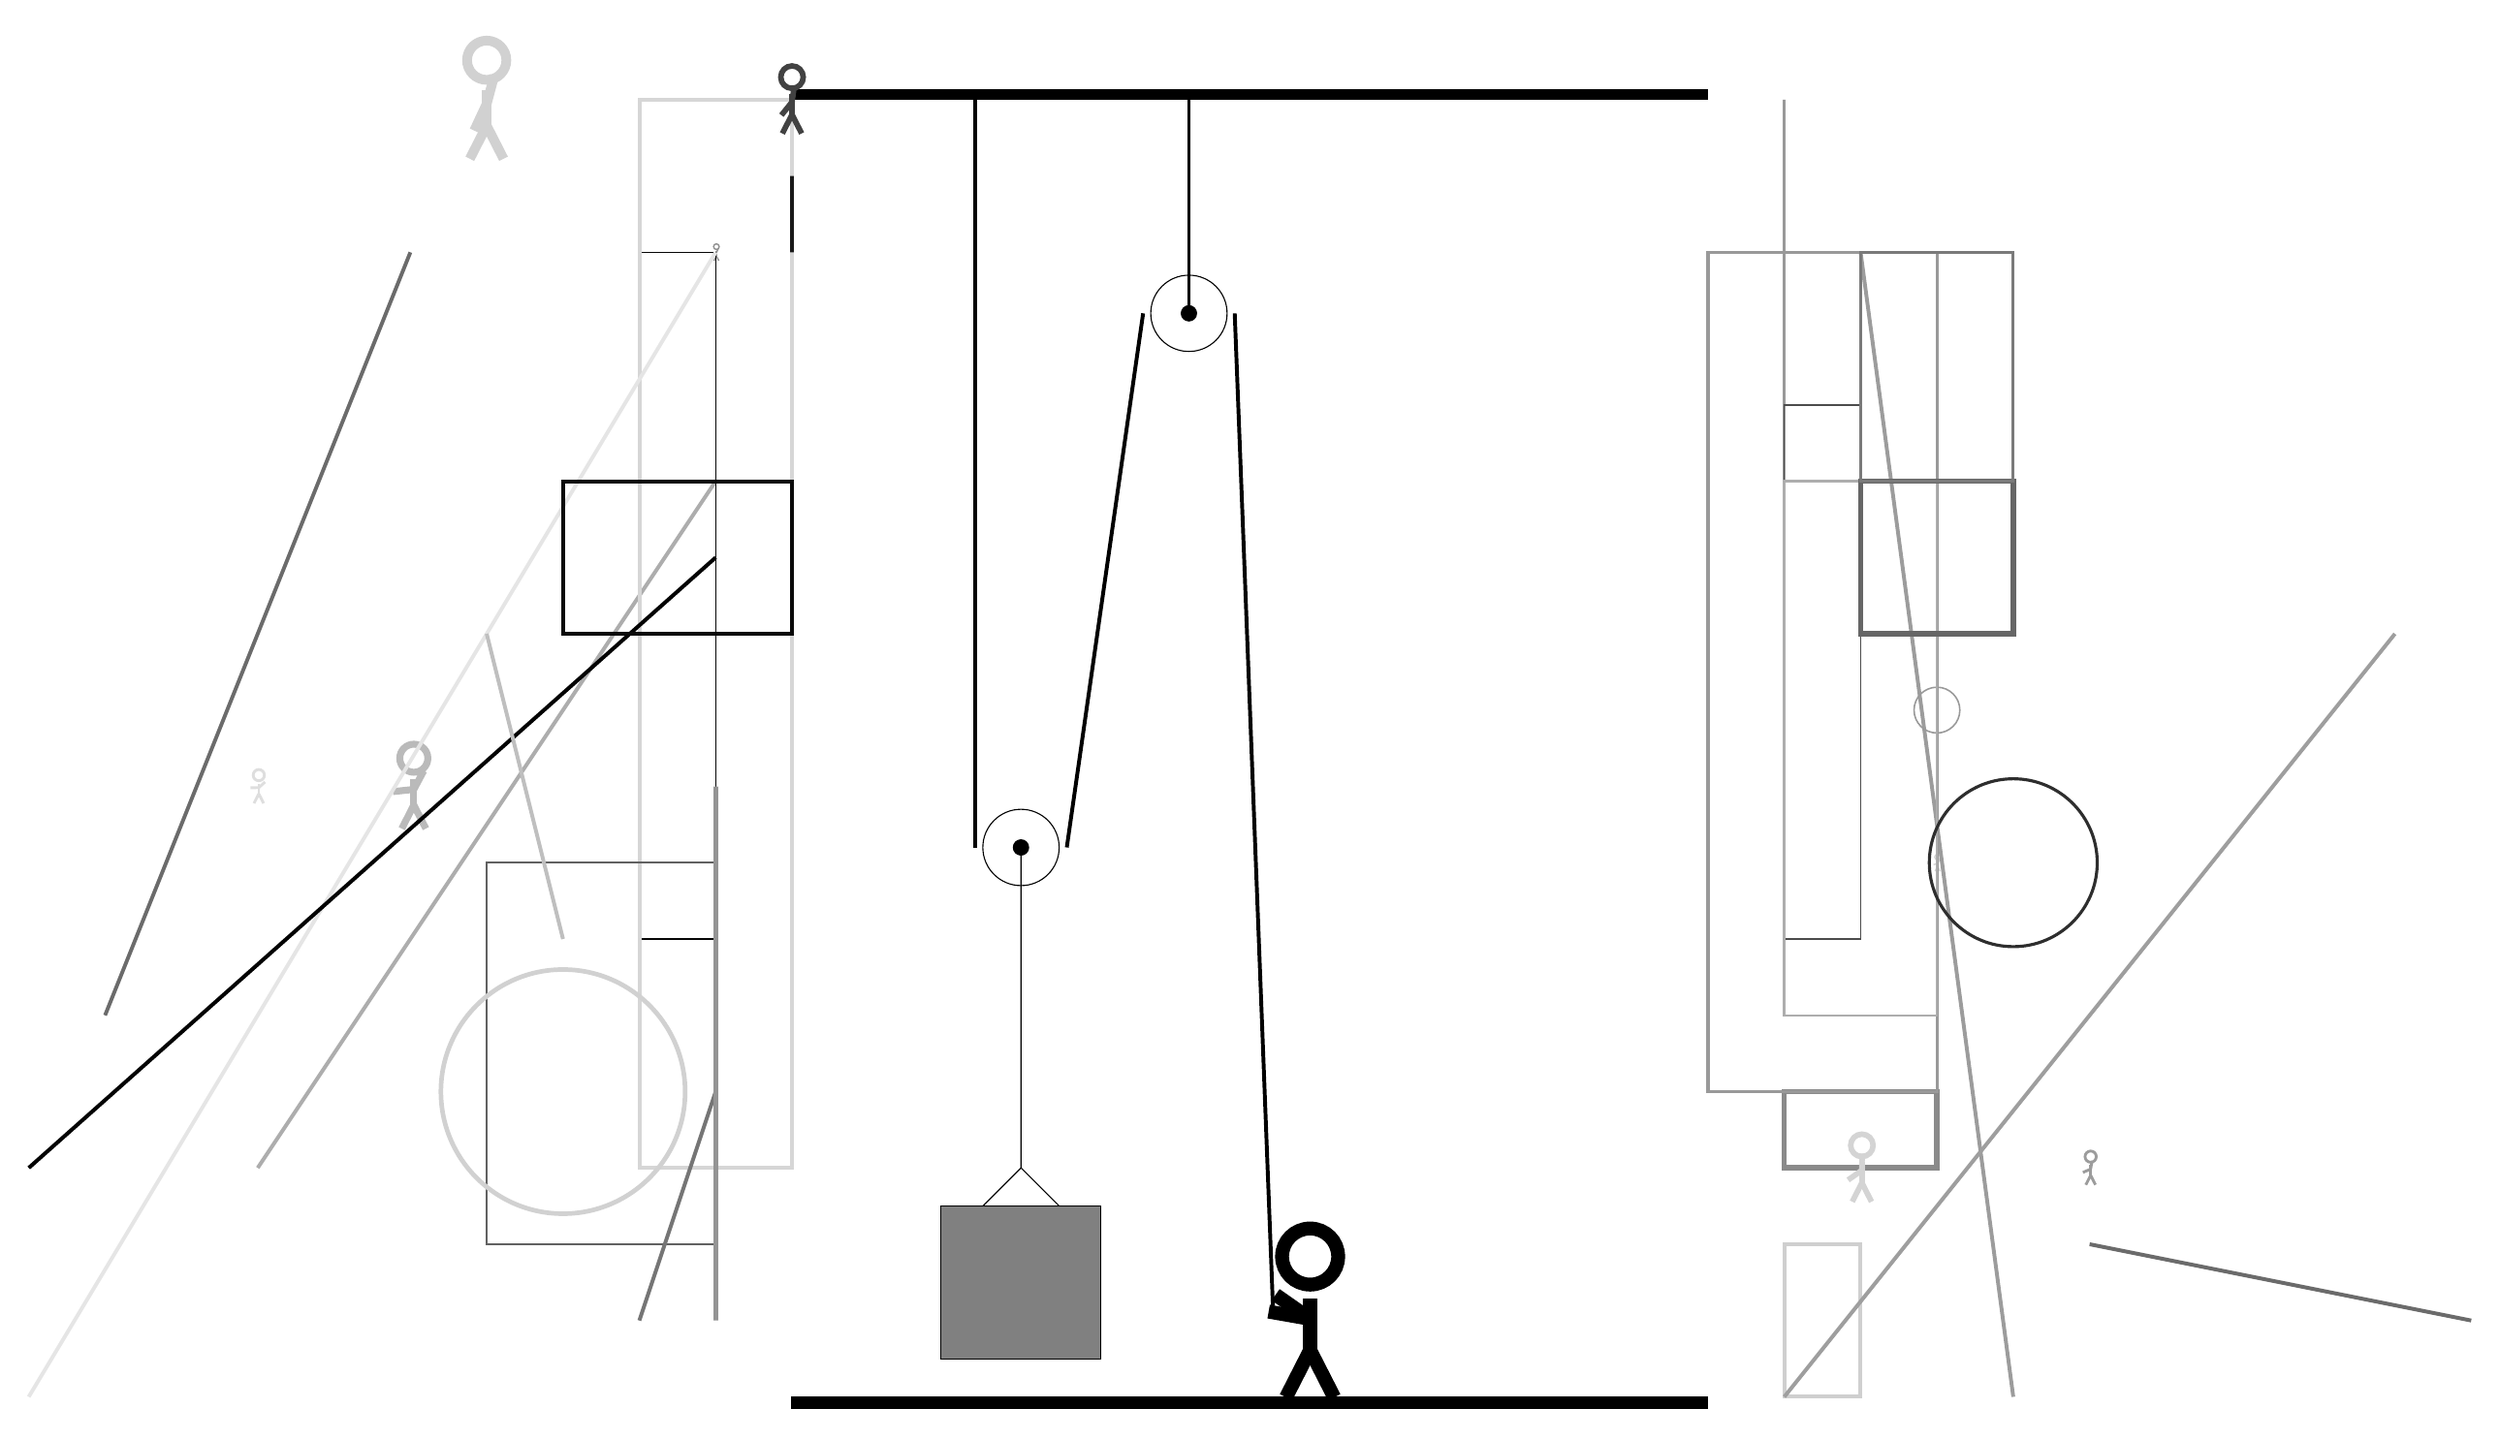
\begin{tikzpicture}
			%%%%% START %%%%%
			
			\draw[fill=black] (-2, 14) rectangle (10, 14.125);
			
			\draw[line width=0.3mm, color=black!40] (11, 3) rectangle (11, 14);
			
			\node[line width=0.4mm, color=black!43] at (-3, 12) {\Strichmaxerl[1][0][67]};
			\draw[line width=0.5mm, color=black!32](-3, 9) -- (-9, 0);
			\draw[line width=0.7mm, color=black!46] (11, 1) rectangle (13, 0);
			\draw[line width=0.5mm, color=black!58](15, -1) -- (20, -2);
			\draw[line width=0.2mm, color=black!98] (-4, 12) rectangle (-3, 3);
			\draw[line width=0.5mm, color=black!16] (-4, 14) rectangle (-2, 0);
			\node[line width=0.2mm, color=black!17] at (13, 4) {\Strichmaxerl[1][20][57]};
			\node[line width=0.7mm, color=black!27] at (-7, 5) {\Strichmaxerl[5][6][62]};
			\draw[line width=0.5mm, color=black!10](-3, 12) -- (-12, -3);
			\draw[line width=0.6mm, color=black!90] (-2, 13) rectangle (-2, 12);
			
			\draw[line width=0.2mm, color=black!62] (-3, 4) rectangle (-6, -1);
			\draw[line width=0.5mm, color=black!54](-3, 1) -- (-4, -2);
			
			\draw[line width=0.5mm, color=black!19] (12, -1) rectangle (11, -3);
			\draw[line width=0.5mm, color=black!39](12, 12) -- (14, -3);
			\draw[line width=0.4mm, color=black!40] (10, 1) rectangle (13, 12);
			
			\draw[line width=0.6mm, color=black!42] (-3, 5) rectangle (-3, -2);
			\node[line width=0.6mm, color=black!18] at (-6, 14) {\Strichmaxerl[7][65][75]};
			\node[line width=0.4mm, color=black!13] at (-9, 5) {\Strichmaxerl[2][1][42]};
			\draw[line width=0.5mm, color=black!99](-3, 8) -- (-12, 0);
			\draw[line width=0.5mm, color=black!58](-7, 12) -- (-11, 2);
			
			\node[line width=0.3mm, color=black!39] at (15, 0) {\Strichmaxerl[2][23][80]};
			\draw[line width=0.2mm, color=black!70] (12, 10) rectangle (11, 3);
			\draw[line width=0.5mm, color=black!96] (-2, 9) rectangle (-5, 7);
			\draw [line width=0.2mm, color=black!40](13, 6) circle (0.3);
			
			\draw[line width=0.3mm, color=black!32] (11, 2) rectangle (13, 9);
			\node[line width=0.4mm, color=black!74] at (-2, 14) {\Strichmaxerl[4][51][82]};
			\node[line width=0.3mm, color=black!17] at (12, 0) {\Strichmaxerl[4][35][89]};
			\draw [line width=0.6mm, color=black!18](-5, 1) circle (1.6);
			\draw[line width=0.5mm, color=black!38](11, -3) -- (19, 7);
			\draw [line width=0.4mm, color=black!82](14, 4) circle (1.1);
			\draw[line width=0.7mm, color=black!60] (12, 9) rectangle (14, 7);
			\draw[line width=0.5mm, color=black!25](-6, 7) -- (-5, 3);
			\draw[line width=0.4mm, color=black!52] (12, 12) rectangle (14, 9);
			
			\draw (3.2, 11.2) circle (0.5);
			\draw[fill=black] (3.2, 11.2) circle (0.1);
			\draw[thick] (3.2, 11.2) -- (3.2, 14);
			
			\draw (1, 4.2) circle (0.5);
			\draw[fill=black] (1, 4.2) circle (0.1);
			
			\draw (1, 4.2) -- (1, 0) -- (0.5, -0.5);
			\draw (1, 0) -- (1.5, -0.5);
			\draw[fill=black!50] (-0.05, -0.5) rectangle (2.05, -2.5);
			
			\draw[line width=0.5mm] (0.4, 14) -- (0.4, 4.2);
			\centerarc[line width=0.5mm](1, 4.2)(180:360:0.6);
			\draw[line width=0.5mm](1.6, 4.2) -- (2.6, 11.2);
			\centerarc[line width=0.5mm](3.2, 11.2)(0:180:0.6);
			\draw[line width=0.5mm](3.8, 11.2) -- (4.3, -1.8);
			
			\node at (4.7, -1.9) {\Strichmaxerl[10][-35][170]};
			
			\draw[fill=black] (-2, -3) rectangle (10, -3.15);
			
			%%%%% END %%%%%
		\end{tikzpicture}
	\end{figure}	
\end{document}